\documentclass{article}

\usepackage{fancyhdr}
\usepackage{extramarks}
\usepackage{amsmath}
\usepackage{amsthm}
\usepackage{amsfonts}
\usepackage{tikz}
\usepackage{graphicx}
\usepackage{float}
\usepackage{listings}
\usepackage{booktabs}

%\usetikzlibrary{automata,positioning}
\usetikzlibrary{shapes, arrows}

%
% Basic Document Settings
%

\topmargin=-0.45in
\evensidemargin=0in
\oddsidemargin=0in
\textwidth=6.5in
\textheight=9.0in
\headsep=0.25in

\linespread{1.1}

\pagestyle{fancy}
\lhead{\hmwkAuthorName}
\rhead{\hmwkClass\ (\hmwkClassInstructor)}
\cfoot{\thepage}

\lstset{
  caption=\lstname,
  %backgroundcolor=\color{lightgray},
  literate={\$}{{\$}}1,
  breaklines=true,
  basicstyle=\ttfamily\small
}

\DeclareMathOperator*{\argmin}{arg\,min}
\renewcommand\headrulewidth{0.4pt}
\renewcommand\footrulewidth{0.4pt}

\setlength\parindent{0pt}

\newcommand{\hmwkTitle}{Utilizing reinforcement learning techniques to play Atari's Breakout}
\newcommand{\hmwkDueDate}{November 3, 2015}
\newcommand{\hmwkClass}{Reinforcement Learning}
\newcommand{\hmwkClassInstructor}{Dr. Itamar Arel}
\newcommand{\hmwkAuthorName}{Andrew Messing, Ben Brock, and Cory Walker}

%
% Title Page
%

\title{
    \vspace{2in}
    \textmd{\textbf{\hmwkTitle}}\\
    \normalsize\vspace{0.1in}\small{Due\ on\ \hmwkDueDate}\\
    \vspace{0.1in}\large{\textit{\hmwkClassInstructor}}
    \vspace{3in}
}

\author{\textbf{\hmwkAuthorName}}
\date{}

\renewcommand{\part}[1]{\textbf{\large Part \Alph{partCounter}}\stepcounter{partCounter}\\}

%
% Various Helper Commands
%

% Alias for the Solution section header
\newcommand{\solution}{ \hfill \break \break \textbf{Solution} \hfill \break \break}

\begin{document}

\maketitle

\pagebreak

\begin{abstract}
  Abstract goes here. Ben, could you take care of this?
\end{abstract}

\section{Introduction}
Some type of introduction goes here. Andrew, could you take care of this?

\section{Breakout and feature extraction}
Andrew's section goes here.

\section{Reinforcement learning}
Ben's section goes here.

\section{Deep reinforcement learning}
Cory's section goes here.
\subsection{Deep Q network}
\subsection{DQN variations}
\subsection{Double DQN formulation}
\subsection{Implementation}
\subsection{Results}
\begin{figure}[H]
  \centering
  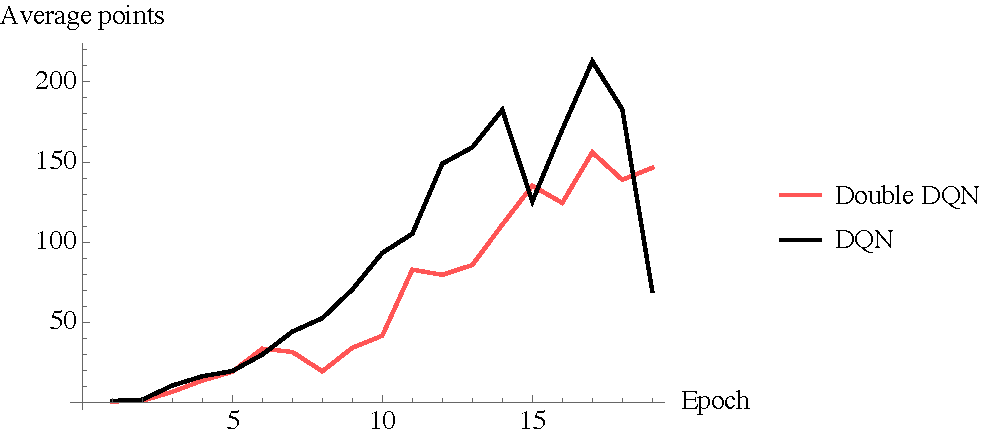
\includegraphics[width=120mm]{dqn_rewardper.pdf}
  \caption{Example figure.}
\end{figure}
Each epoch takes about an hour. Stopped after $\sim 20$ hours.\\

\section{Design challenges}
Put design challenges here.

\section{Summary}
A summary goes here.

%\section{Appendix}
%\begin{center}
  %\lstinputlisting{/Users/cwalker32/Documents/LaTeX/ece_517/proj2/et.m}
%\end{center}


\pagebreak

\end{document}
